\documentclass[preprint]{elsarticle}

\usepackage{lineno,hyperref}
\usepackage{graphicx}
\usepackage{amsmath}
\usepackage[linesnumbered,ruled]{algorithm2e}
\modulolinenumbers[5]

\journal{Expert Systems with Applications}

%%%%%%%%%%%%%%%%%%%%%%%
%% Elsevier bibliography styles
%%%%%%%%%%%%%%%%%%%%%%%
%% To change the style, put a % in front of the second line of the current style and
%% remove the % from the second line of the style you would like to use.
%%%%%%%%%%%%%%%%%%%%%%%

%% Numbered
%\bibliographystyle{model1-num-names}

%% Numbered without titles
%\bibliographystyle{model1a-num-names}

%% Harvard
%\bibliographystyle{model2-names.bst}\biboptions{authoryear}

%% Vancouver numbered
%\usepackage{numcompress}\bibliographystyle{model3-num-names}

%% Vancouver name/year
%\usepackage{numcompress}\bibliographystyle{model4-names}\biboptions{authoryear}

%% APA style
%\bibliographystyle{model5-names}\biboptions{authoryear}

%% AMA style
%\usepackage{numcompress}\bibliographystyle{model6-num-names}

%% `Elsevier LaTeX' style
\bibliographystyle{elsarticle-num}
%%%%%%%%%%%%%%%%%%%%%%%

\begin{document}

\begin{frontmatter}

\title{Origin based Order Independent Association Rule Mining using multiple OIMASP tree\tnoteref{mytitlenote}}
\tnotetext[mytitlenote]{Fully documented templates are available in the elsarticle package on \href{http://www.ctan.org/tex-archive/macros/latex/contrib/elsarticle}{CTAN}.}

%% Group authors per affiliation:
\author{Elsevier\fnref{myfootnote}}
\address{Radarweg 29, Amsterdam}
\fntext[myfootnote]{Since 1880.}

%% or include affiliations in footnotes:
\author[mymainaddress,mysecondaryaddress]{Elsevier Inc}
\ead[url]{www.elsevier.com}

\author[mysecondaryaddress]{Global Customer Service\corref{mycorrespondingauthor}}
\cortext[mycorrespondingauthor]{Corresponding author}
\ead{support@elsevier.com}

\address[mymainaddress]{1600 John F Kennedy Boulevard, Philadelphia}
\address[mysecondaryaddress]{360 Park Avenue South, New York}

\begin{abstract}
We discuss the problem of mining association rules in the transaction dataset. The previous approach(MASP \cite{oldmasp}) is dependent on the order of items in the dataset. We proposed a novel method which is order independent and also takes into consideration the origin of items to calculate unbiased support and confidence values. Five datasets are used for comparison. The results show that the new approach outperforms the previous approach concerning the number of association rules and length of the longest association rule. On an average, the proposed method requires more computational resources in terms of time. We believe that the extra information extracted using new method compensates for the increase in time complexity as compared to MASP approach. The algorithm produces multiple trees which can be helpful in the visual analysis of data.
\end{abstract}

\begin{keyword}
Data Mining \sep Association Rule Mining \sep MASP \sep Support 
\sep Confidence \sep Transaction Database \sep Transaction
\end{keyword}

\end{frontmatter}

\section{Introduction}
Association rule mining is a rule-based machine learning procedure to find interesting patterns in the transaction database based on individual and conditional frequencies. In the conventional approach, two phases are involved in generating rules. In the first phase, all the itemsets are generated and in-frequent itemsets are pruned. In the second phase, rules are derived from those frequent itemsets. An association rule e.g. \{bread, milk\} $\Rightarrow$ \{butter\} in market basket analysis means if one purchase bread and milk together it is highly likely that they will also buy butter. Apart from market basket analysis, association rule mining is useful in intrusion detection, bioinformatics, and many other applications.

In 2014 O. M. Soyal, et al. \cite{oldmasp} proposed a new approach to extract mostly associated sequential patterns (MASPs) using less computational resources in terms of time and memory while generating a long sequence of patterns that have the highest co-occurrence.

\begin{figure*}
\begin{center}
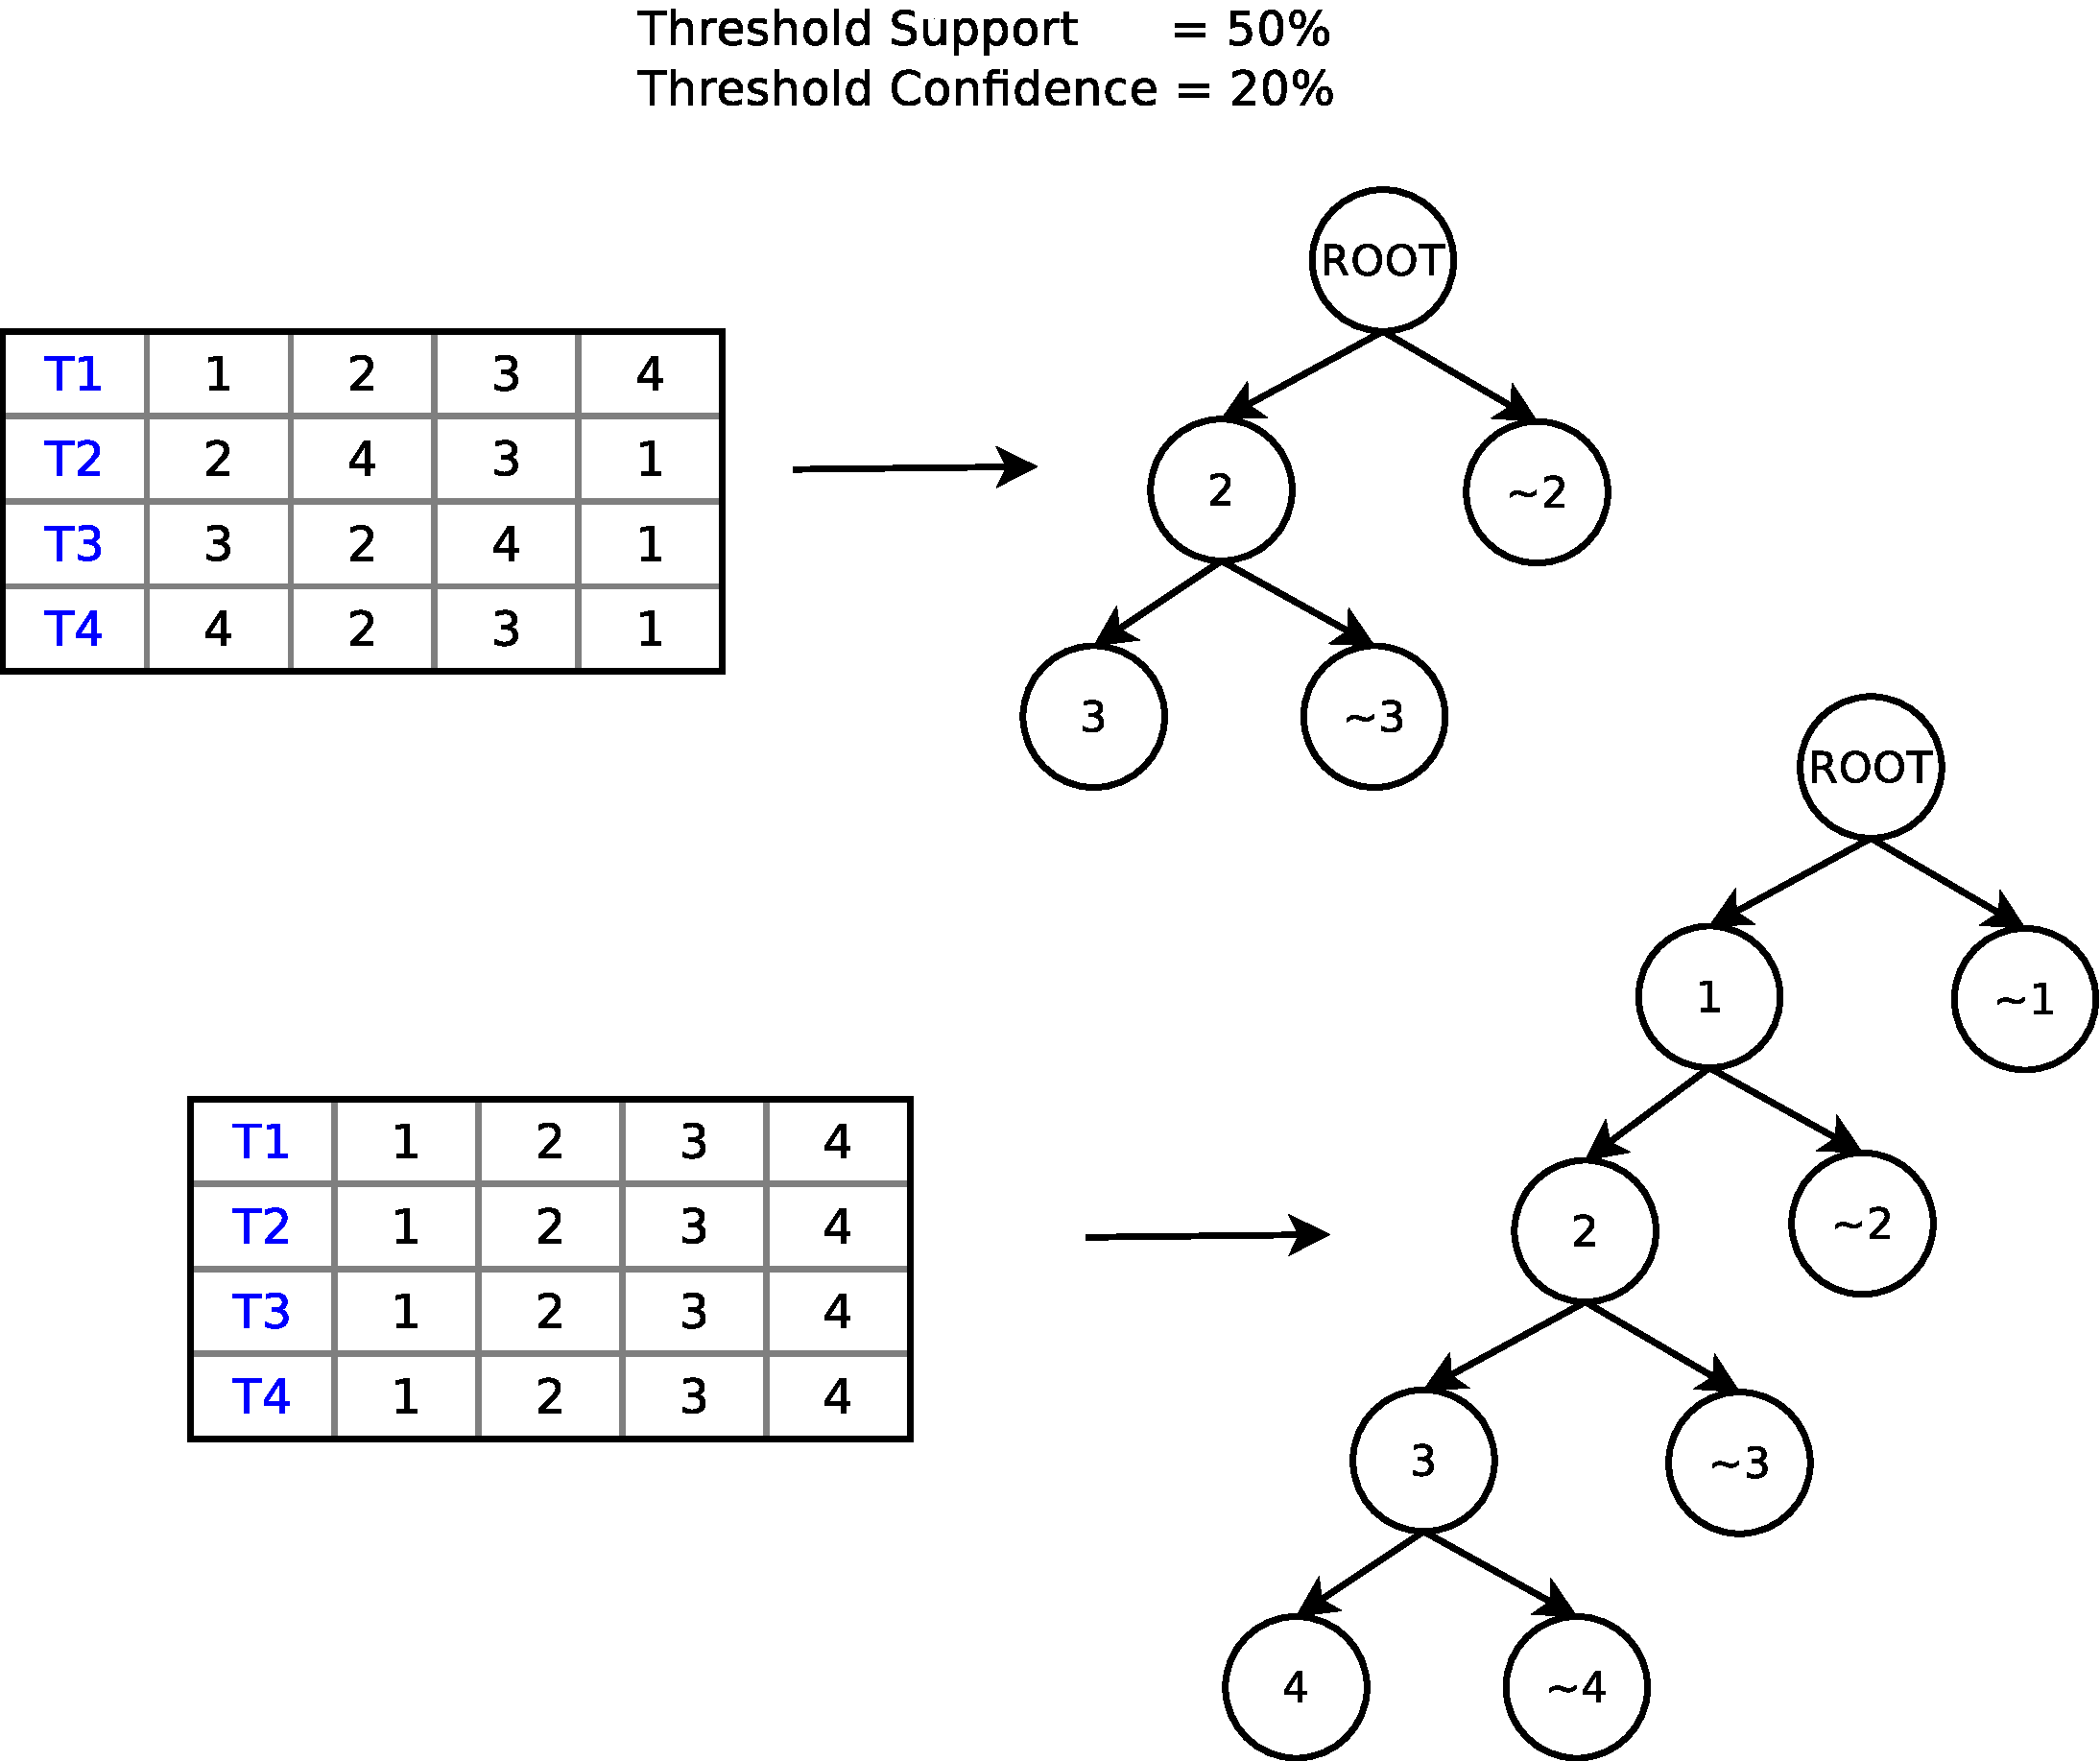
\includegraphics[scale=0.30]{pdf/firstimprove}
\end{center}
\caption{Differnt \emph{MASP} tree for the same dataset}
\label{Fig 12}
\end{figure*}

This approach may produce different outcomes if we change the order of items in transactions. Figure \ref{Fig 12} shows this issue. In Figure \ref{Fig 12} the MASP tree changes with the change in the order of items in transactions for threshold support 0.50 and threshold confidence 0.20. We propose an approach which is order independent. An association rule of the form \textit{A} $\Rightarrow$ \textit{B} must satisfy the threshold support and threshold confidence i.e. probability of occurrence of \textit{A} and \textit{B} together must surpass threshold support, and the likelihood of occurrence of \textit{B} in transactions containing \textit{A} must be greater than or equal to threshold confidence. It means, to calculate support and confidence, it is required to traverse complete transaction database. What if an item appears for the first time in the $ ith $ transaction? It is biased to take the entire dataset for calculating support and confidence for the rules containing that particular item. So to generate all rules containing a particular item x, it is reasonable to ignore all transactions(for calculating support and confidence) that come before the transaction in which that particular item appears for the first time. Taking into account the origin of the item is the second contribution. Embedding these two changes to the Omer M. Soyal \cite{oldmasp} approach is the basis of our research.\\
\\
Our contributions
\begin{enumerate}[1)]
\item Make the MASP(\cite{oldmasp}) algorithm order independent.
\item Consider the origin of items for calculating unbiased support and confidence.
\end{enumerate}

\section{Related works}
In 1994 R. Agrawal, et al. published non-trivial algorithm(Apriori) \cite{fastapriori} for finding association rules in large databases of the sales transaction. Apriori algorithm produces association rules in two phases. In the first phase, all the itemsets are generated, and infrequent itemsets are pruned. In the second phase, rules are derived from those frequent itemsets. This algorithm first finds frequent itemsets of length 1 then frequent itemsets of length 2 using frequent itemsets of length 1 and so on until generation of all frequent itemsets. This algorithm performs better than the previously known fundamental algorithms AIS \cite{ais}, SETM \citep{setm}. In 1996 Fukuda, et al. \cite{2darules} proposed an approach to find two-dimensional association rules. A state in this scenario is of the form ((\textit{X}, \textit{Y}) $\in$ \textit{P}) $\Rightarrow$ (\textit{Z} = z) where \textit{X} and \textit{Y} are numeric attributes, \textit{P} is a subspace of 2-D plane, and \textit{Z} is a boolean attribute i.e. z can be either true or false. E.g. (\textit{Age} $\in$ [30, 50] $\wedge$ \textit{Balance} $\in$ [10$^{5}$, 10$^{6}$]) $\Rightarrow$ (\textit{CardLoan} = yes). It means if a bank user age and balance lies in the given subspace it is very likely that they will use card loan. This approach works for specific types of structured data. R. Feldman, et al.(1997) \cite{massociation} introduced the notion of maximal association rules. These are the rules extracted from frequent maximal itemsets. Frequent maximal itemsets are those itemsets which appear just once among all the transactions. It is useful in finding association rules containing negated attributes. As an example, a rule \{milk, $\neg$bread\} $\Rightarrow$ \{$\neg$butter\} contains negated attributes. It means if a user purchases milk but not bread then the probability that the user will not buy butter is very high. This approach helps to capture inference rules which might be lost using regular associations. Till now items in transaction databases were treated uniformly. In 1998 C.H. Cai, et al. \cite{weightedassociation} gave an approach to find association rules which take into account weight(importance) of items in transaction databases. 

FP-Growth algorithm(2000) \cite{fpgrowth} also operates in two phases. The second phase is same as apriori. FP-Growth does not generate candidate frequent itemsets. First, it creates a tree(FP-Tree) and then finds frequent itemsets. This algorithm is about an order of magnitude faster than the Apriori algorithm. Lin, Weiyang, et al. \cite{Lin2002} proposed an approach that uses association rule mining for collaborative recommender systems. This approach does not require threshold support value. Instead, based on the number of rules(given) to be generated, threshold support is decided by the system. Thus it reduced the running time and produced enough rules for good recommendation. In 2004, F. Conen, et al. \cite{ptree} proposed two structures(T-Trees and P-Trees) along with associated algorithms which offer significant advantages w.r.t storage and execution time. In 2005, K. G. Srinivasa, et al. \cite{genetic} took advantage of genetic algorithms principles(\cite{Srinivas:1994:GAS}) to generate large itemsets within dynamic transaction database. Their algorithm was better than the pre-existing FUP and E-Apriori concerning execution time and scalability. If transaction database is static, then computations will be way easy. In other scenario transaction database keeps on changing at high speed leading to change in data distribution. Hence it will be difficult to apply previously mentioned Association Rule Mining techniques. Jiang, et al.(2006) \cite{dynamicarm} proposed ways to address issues such as data processing model, memory management, etc. when performing association rule mining for stream data.

In 2006, G. Chen, et al. \cite{classify} used association rule mining for solving classification problems. It gave satisfactory results when compared to then existing classification algorithms like C4.5, CBA, SVM, NN. Modification of the conventional algorithm(apriori) was done \cite{bookrecommend} for building book recommendation system, based on the data obtained from historical data of university library. Association rules having low support and high confidence are exception rules. In 2008 D. Taniar, et al. \cite{exceptionrules} proposed a new approach to finding exception rules. In the first phase, generate candidate exception rules and based on exceptionality measure, obtain the final ruleset. The quality of association rules depends on the threshold value of support and confidence. R.J. Kuo, et al.(2011) \cite{swarmarm} proposed an approach to find best threshold values which can produce quality rules. It gave promising results when compared to the genetic algorithm. Cloud computing provides an efficient and cheap way to store and analyze data. In 2011, L. Li, et al. \cite{cloudarm} proposed an effective strategy to perform association rule mining(frequent itemset mining) in cloud computing environment. 

In the first phase of Apriori \cite{fastapriori} algorithm, all the itemsets are generated, and infrequent itemsets are pruned. The modified algorithm(2012) \cite{minmizcandidt} reduces the burden of pruning step, since it generates fewer candidate itemsets. In 2013, Tseng, et al. \cite{Tseng:2013:MFI} proposed an approach(Hierarchical Partitioning) to perform frequent itemset mining in big databases. It uses Frequent Pattern List(FPL) data structure. FPL partitions the transaction database into a set of sub-databases before performing frequent itemset mining. With the passage of time Association Rule Mining find its role in many applications. J. Nahar, et al.(2013) \cite{armheart} proposed a way to detect factors that can contribute to heart diseases in males and females. High Utility Itemset mining is used to find all the itemsets that generate at least threshold profits. It takes into account quantity of items and benefits. It is useful in many applications such as stock market prediction and retail market data analysis. Before mining high utility itemset it is required to set the threshold value of profits(min\_util). It's difficult for users to set an appropriate value of min\_util. Low value leads to too many itemsets. On the other side, high value results into low or no itemsets at all. Cheng, et al. \cite{Wu:2012:MTH} introduced a new framework top-k high utility itemset mining, where k is the number of these itemsets to be mined. They proposed an efficient algorithm named TKU (Top-K Utility itemsets mining) for mining high utility itemset without setting any threshold value. Before 2014 there were many algorithms available to perform high utility itemset mining. These algorithms generate a significant number of candidate itemsets that diminishes the mining performance. Yun, et al.(2014) \cite{Yun:HUI} proposed an approach which prunes candidate itemsets efficiently. They also proposed a tree data structure which captures entire transaction database in a single pass. Their approach outperforms the state of the art tree based algorithms in runtime. To enhance the quality of association rule mining, it may be worthy to include factors such as value utility, temporal, etc. G. Maragatham, et al.(2015) \cite{utarm} have proposed an efficient algorithm which combines both utility and temporal time periods for mining extraordinary association rules. Their results show that UTARM(Utility-Based Temporal Association Rule Mining) algorithm efficiently discovers the utility-oriented temporal association rules. In 2016 O. M. Soysal, et al. \cite{sparseds} proposed a data structure for sparse memory allocation for parallel and sequential data mining. They have used this data structure on apriori-TID, MASP-tree, and FP-growth algorithms to reduce memory allocation cost. They concluded that the speed-up in apriori-TID is more than FP-growth and the modified MASP algorithm becomes 3.42 times faster than the old implementation \cite{oldmasp}.

\section{Model}
Let $ I $ be a universal set of items. A single transaction($ \tau $) is a non-empty subset of universal itemset($ I $). Mathematically, $ \tau = \lbrace item : item$ $\epsilon $ $ I \rbrace$. A transaction database($ \Gamma $) is a collection of such transactions. A rule of the form $ X \Rightarrow  Y $ must satisfy $ support(X \Rightarrow Y) $ $ \geq $ $ \tau _{s} $(threshold support) and $ confidence(X \Rightarrow Y) $ $ \geq $ $ \tau _{c} $(threshold confidence) where $ X $ and $ Y $ are non-empty subsets of $ I $ and $ X $ $ \cap $ $ Y $ $ = \phi $. $ support(X \Rightarrow Y) $ is defined as the probability of occurrence of $ X $ and $ Y $ together in the transaction database($ \Gamma $). Mathematically, $ support(X \Rightarrow Y) $ $ = $ $ \frac{Count(X \cup Y)}{Count(\phi)} $ where $ Count(Z) $ is the number of transactions which are superset of $ Z $. $ confidence(X \Rightarrow Y) $ is the probability of occurrence of $ Y $ in those transactions of $ \Gamma $ which contains $ X $ or $ confidence(X \Rightarrow Y) $ $ = $ $ Probability(Y  \vert  X) $ $ = $ $ \frac{Count(X \cup Y)}{Count(X)} $. The values of threshold support($ 0 \leq \tau _{s} \leq 1 $) and threshold confidence($ 0 \leq \tau _{c} \leq 1 $) are selected before performing association rule mining.

First, we will explain how to generate $ OIMASP $ tree before taking into account the origin of the item in $ \Gamma $. Some of the terminologies that will be helpful in understanding the algorithm.

\begin{enumerate}[1.]
\item \textbf{Transaction($ \tau $):} It is a subset of universal itemset.
\item \textbf{Transaction Dataset($ \Gamma $): } A compilation of many transactions. Constraints imposed on  transaction dataset are
\begin{enumerate}[a)]
\item Every row(transaction) in the transaction database must have the same number of items.
\item No duplicate items are allowed in rows of $ \Gamma $.
\end{enumerate}

\begin{figure}
\begin{center}
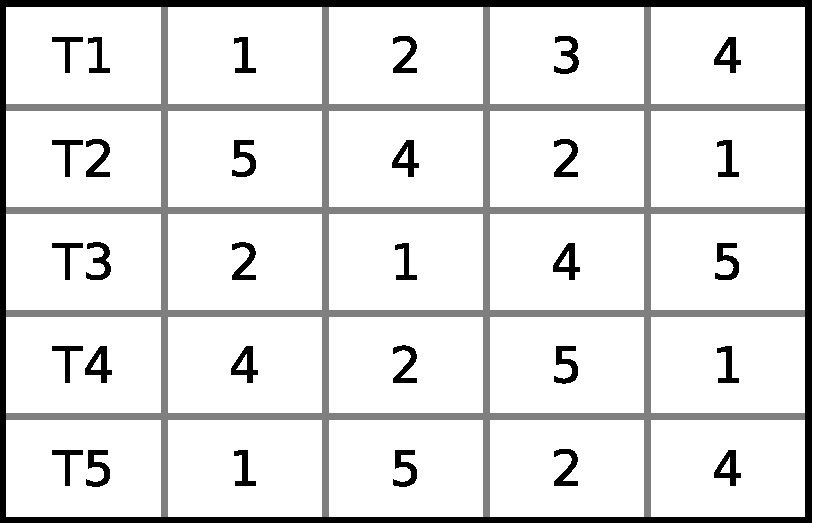
\includegraphics[scale=0.3]{pdf/validtrans}
\end{center}
\caption{Valid Transaction Dataset}
\label{Fig 1}
\end{figure}

\begin{figure}
\begin{center}
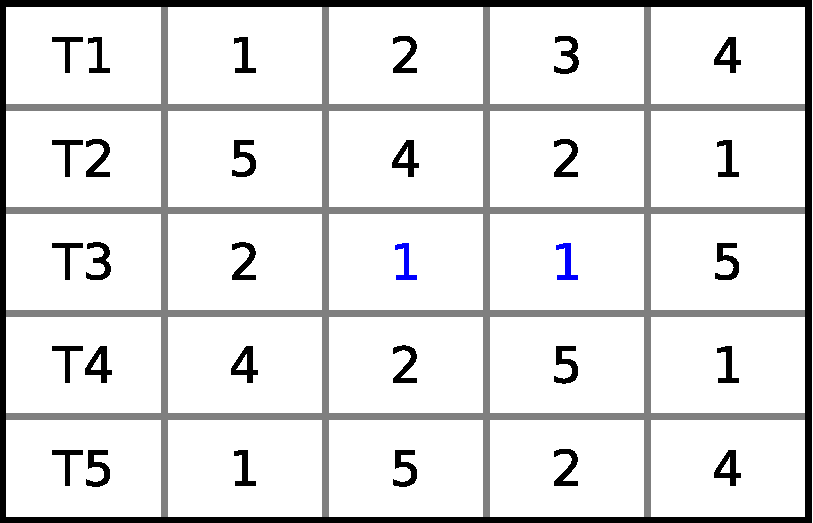
\includegraphics[scale=0.3]{pdf/invalidtrans}
\end{center}
\caption{Invalid Transaction Dataset}
\label{Fig 2}
\end{figure}

Transaction database \ref{Fig 1} is valid, and \ref{Fig 2} is invalid(duplicate items(blue color) in \emph{T3}).

\item \textbf{OIMASP:} A sequence of items $ I = \{I_{1}, I_{2}, I_{3}, ..........., I_{n}\} $ will be an \textbf{OIMASP} iff $ \forall j $  $ \in $ $ {1, 2, ...., n} $ the subset $ I' = \{I_{1}, I_{2}, ......., I_{j}\} $ satisfies the following
\begin{enumerate}[i)]
\item $ support(I') \geq  \tau _{s} $
\item $ P(I_{j} \vert I_{1}, I_{2}, ......., I_{j-1}) \geq \tau _{c} $
\item $ P(I_{j} \vert I_{1}, I_{2}, ......., I_{j-1}) $ is maximum.
\end{enumerate}

\item \textbf{Shuffle:} It is a function which takes transaction dataset, and an item as inputs and returns shuffled transaction dataset or \textbf{Shuffle}($ \Gamma $, \emph{I}) $ \rightarrow $ $ \Gamma _{shuffled} $. Shuffling is done in two steps
\begin{enumerate}[i)]

\item $ \forall $ rows, if the specified item($ I $) is present in the row then perform swapping to bring that item to the first column(Figure \ref{Fig 3}).
\item Shuffle rows until there is no row left which contains item $ I $ and appears below row which do not have item $ I $(Figure \ref{Fig 3}).
\end{enumerate}

\begin{figure*}
\begin{center}
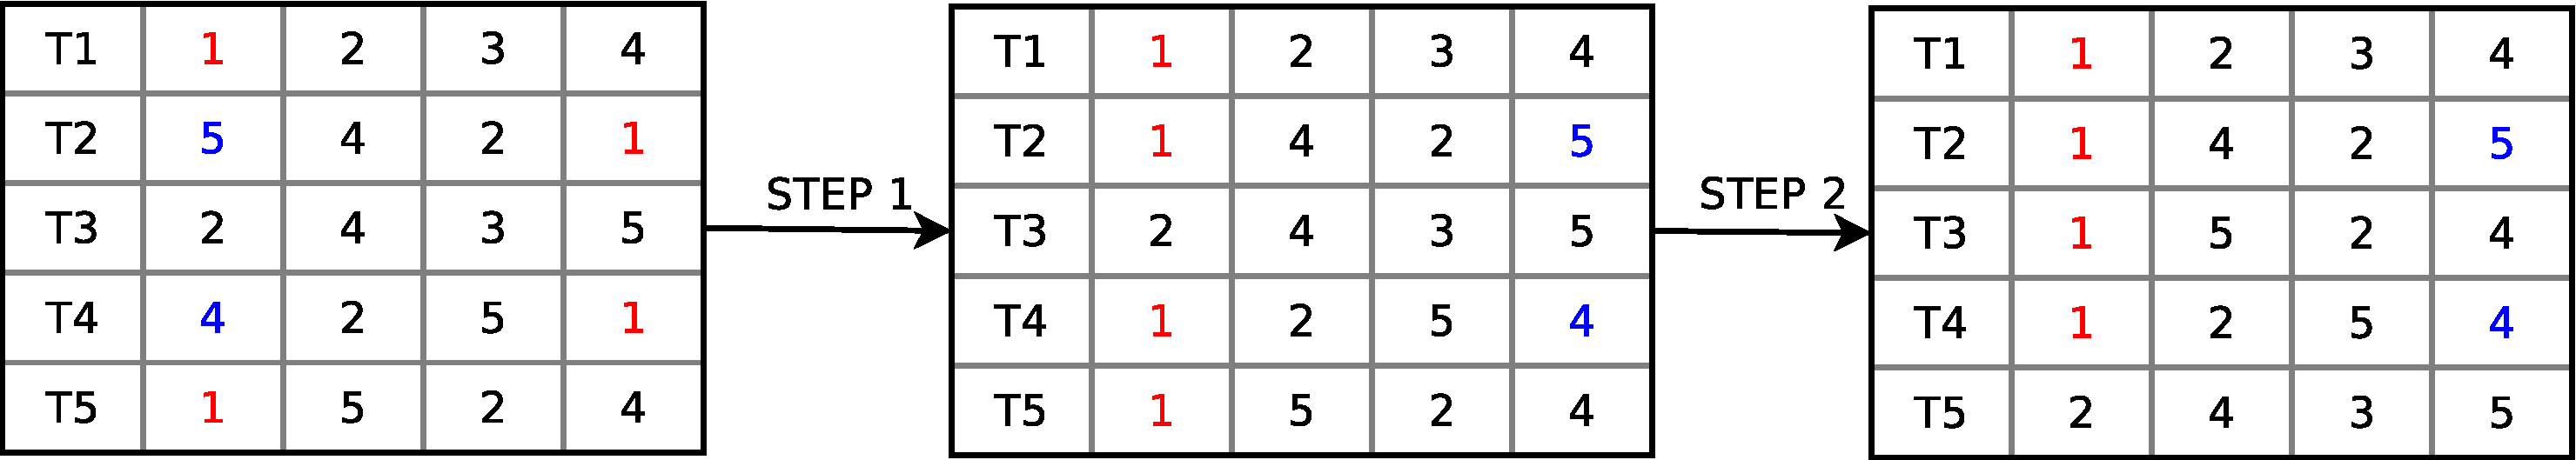
\includegraphics[scale=0.242]{pdf/shuffle}
\end{center}
\caption{Shuffling of dataset as per item \textbf{1}}
\label{Fig 3}
\end{figure*}

\begin{figure*}
\begin{center}
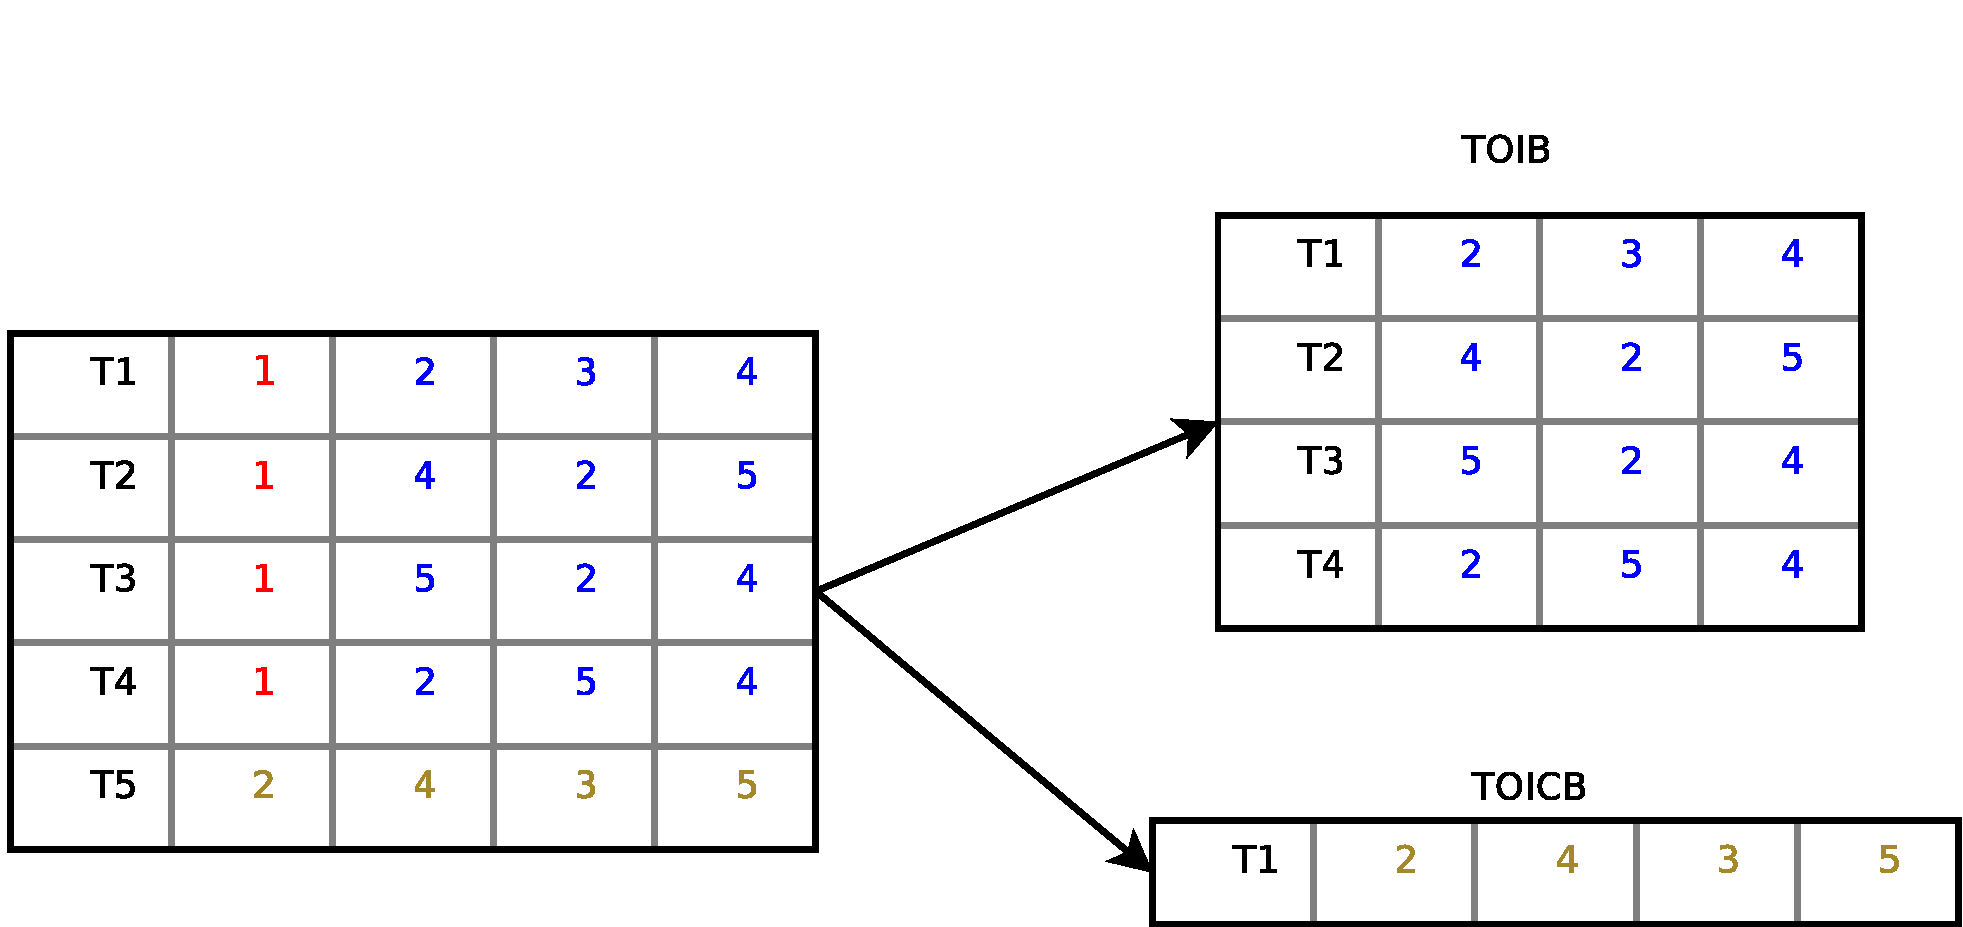
\includegraphics[scale=0.3]{pdf/tbtcb}
\end{center}
\caption{Splitting of $ \Gamma _{shuffled} $ into temporary order independent block and counter block}
\label{Fig 4}
\end{figure*}

\item Temporary Order Independent Block(\textbf{TOIB})\textbf{:} After shuffling is done w.r.t the specified item, first obtain a subset of $ \Gamma _{shuffled} $ by taking transactions having specified item and then in the second step remove the first column. This newly received dataset is \textbf{TOIB}(Figure \ref{Fig 4}).

\item Temporary Order Independent Counter Block(\textbf{TOICB})\textbf{:} After shuffling is done w.r.t the specified item, the subset of $ \Gamma _{shuffled} $ obtained by taking transactions not having specified item is \textbf{TOICB}(Figure \ref{Fig 4}).

\item \textbf{Frequency Table:} A table which stores the frequency of items. In Figure \ref{Fig 5} the frequency table corresponding to the transaction table is shown on the right. $ f_{max} $ is the maximum frequency in the frequency table. $ I_{max} $ is the item having frequency $ f_{max} $. If multiple items have frequency $ f_{max} $, then $ I_{max} $ can be any of them.

\begin{algorithm}
    \SetKwInOut{Input}{Input}
    \SetKwInOut{Output}{Output}

    \underline{function FindDataset} $ (\Gamma, OIMASP, j = 1) $\;
    \Input{A transaction dataset $ \Gamma $, $ OIMASP $ sequence}
    \Output{Dataset associated with the $ OIMASP $ }
    \If{$ j > $ $ sizeof(OIMASP) $}
      {
        return $ \Gamma $
      }     
    \eIf{negation is present on $ jth $ item of $ OIMASP $}
      {
        $ temp \leftarrow TOICB(\Gamma, OIMASP[j]) $\;
		return $ FindDataset(temp, OIMASP, j+1) $
      }
      {
		$ temp \leftarrow TOIB(\Gamma, OIMASP[j]) $\;
		return FindDataset$(temp, OIMASP, j+1)$
      }      
    \caption{Algorithm to obtain the dataset associated with an $ OIMASP $ sequence}
\end{algorithm}

\end{enumerate}

\section{Algorithms}

\subsection{How to generate OIMASP tree?}
In this section, we have proposed an algorithm($ OIMASP $)[modified version of MASP \cite{oldmasp}] which is independent of the ordering of items in transactions.

\begin{figure}
\begin{center}
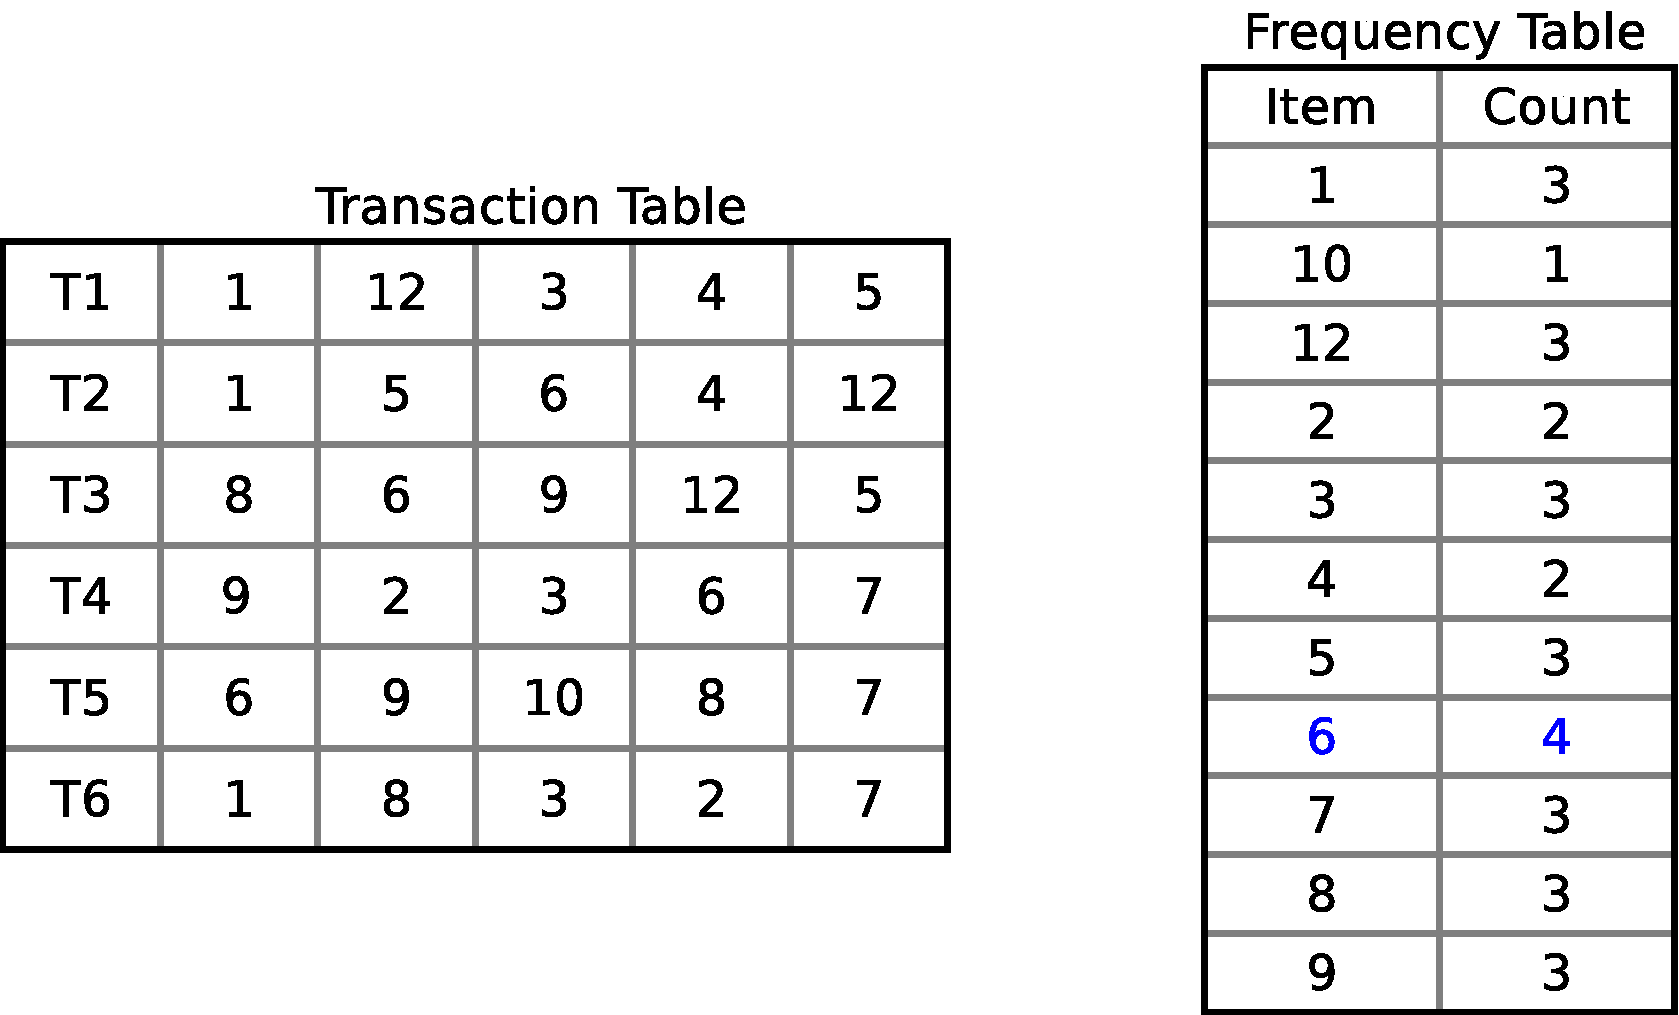
\includegraphics[scale=0.25]{pdf/itemfreq}
\end{center}
\caption{Transaction table on the left and items and their frequencies on the right}
\label{Fig 5}
\end{figure}

\begin{algorithm}
    \SetKwInOut{Input}{Input}
    \SetKwInOut{Output}{Output}

    \underline{function OIMASP} $ (\Gamma_{current}, Node) $\;
    \Input{A transaction dataset $ \Gamma_{current} $ associated with the $ Node $ of the $ OIMASP $ tree}
    \Output{An $ OIMASP $ tree}
    Obtain the frequency table of $ \Gamma_{current} $\\
    Find the item $ I_{max} $ having maximum frequency $ f_{max} $\\
    \If{(support = $ \dfrac{f_{max}}{\vert \Gamma \vert} $) $ < \tau _{s} $}
      {
        return $ Node $
      }     
    \If{(confidence = $ \dfrac{f_{max}}{\vert \Gamma_{current} \vert} $) $ < \tau _{c} $}
      {
        return $ Node $
      }
    Add a node on the left side of $ Node $ say $ Node_{left} $ and store $ I_{max} $ in it\\
    
    Add a node $ Node_{right} $ on the right side of $ Node $ and store  $ \sim I_{max} $ in it\\
    
    $ \Gamma_{left} = TOIB(\Gamma_{current}, I_{max}) $\\
    $ \Gamma_{right} = TOICB(\Gamma_{current}, I_{max}) $\\
    
    $ OIMASP(\Gamma_{left}, Node_{left}) $\\
    $ OIMASP(\Gamma_{right}, Node_{right}) $\\
    return $ Node $
    \caption{Algorithm to generate $ OIMASP $ tree. $ \Gamma $ is the input transaction database, $ \vert \Gamma \vert $ is the number of rows in $ \Gamma $, $ \tau_{s} $ is the threshold support, and $ \tau_{c} $ is the threshold confidence.}
\end{algorithm}

\begin{figure*}
\begin{center}
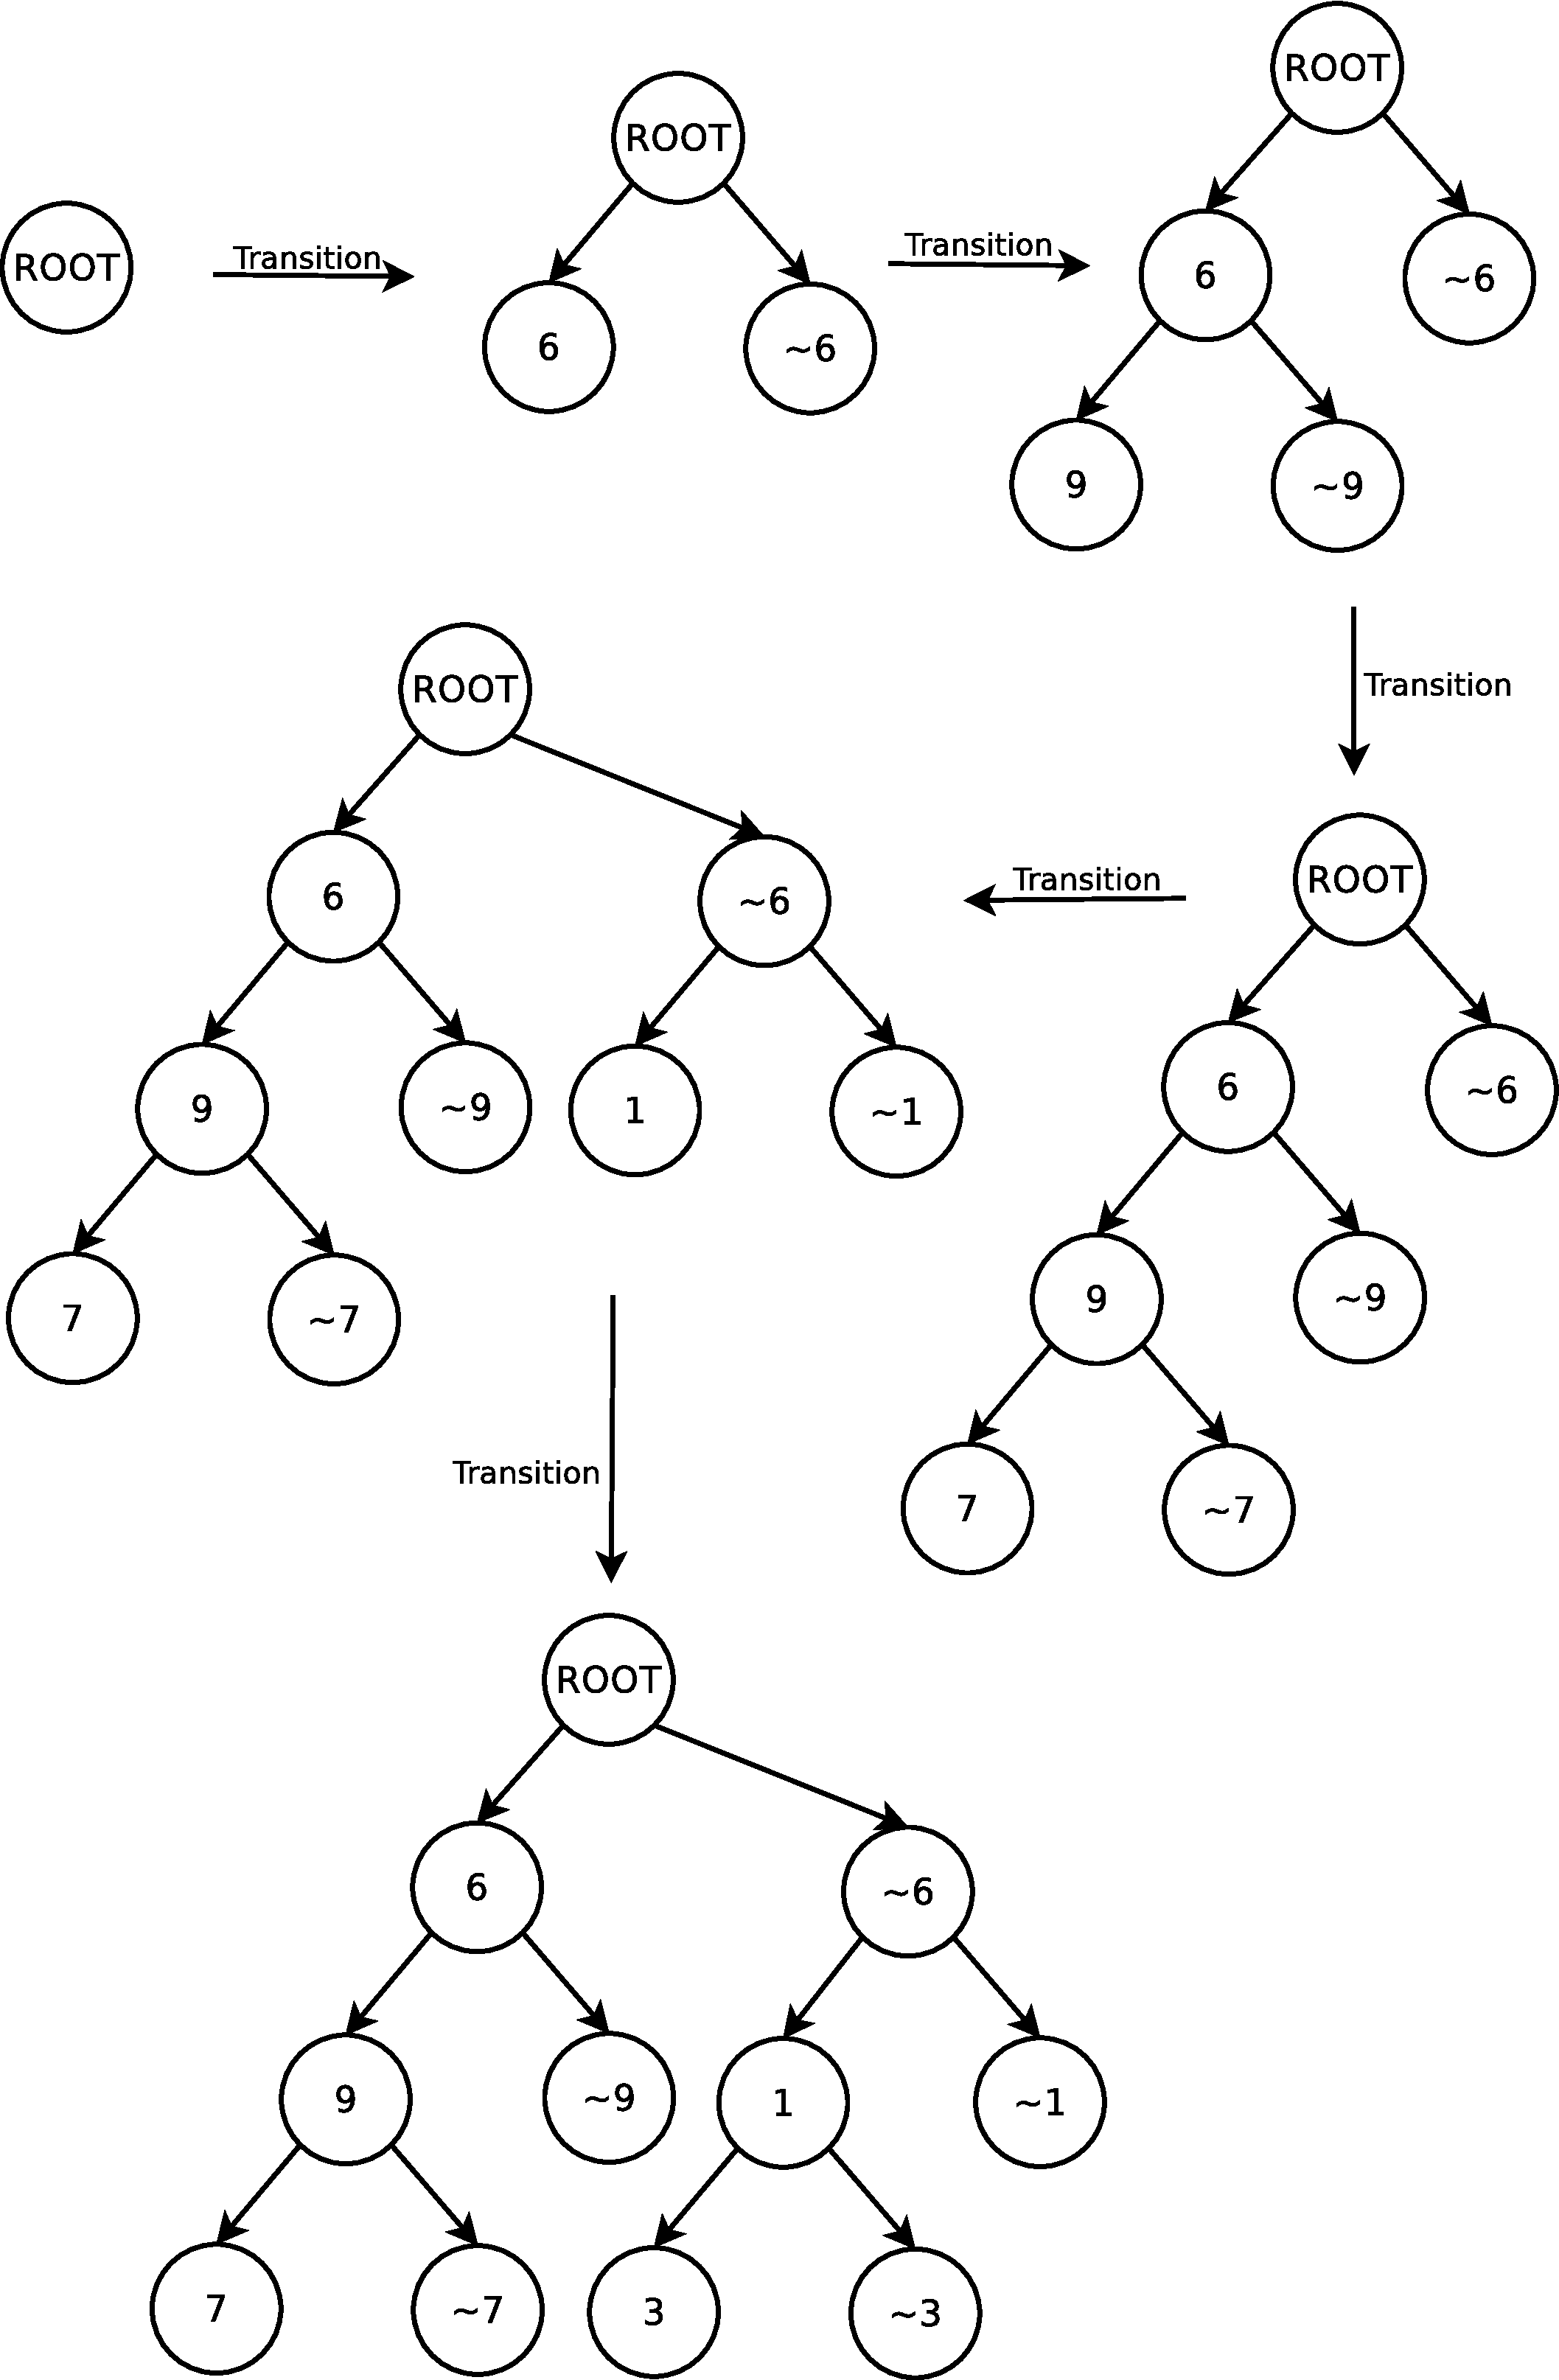
\includegraphics[scale=0.3]{pdf/transition}
\end{center}
\caption{Generation of OIMASP tree as the algorithm proceeds}
\label{Fig 6}
\end{figure*}

If we apply the $ OIMASP $ algorithm for the transaction dataset shown in Figure \ref{Fig 5}, threshold support($ \tau _{s} $) $ = 0.2 $ and threshold confidence($ \tau _{c} $) $ = 0.3 $, we will get the final $ OIMASP $ tree in series of transitions as shown in Figure \ref{Fig 6}. The OIMASP algorithm starts with a root node(Figure \ref{Fig 6}) having data $ \Gamma $. The item having maximum frequency is 6, and it satisfies the threshold support and threshold confidence conditions. Therefore two nodes are added, 6 on the left and $ \sim $ 6 on the right and data associated with 6 and  $ \sim $ 6 are TOIB and TOICB respectively w.r.t. item 6 and data $ \Gamma $. The same will be repeated for 6 and $ \sim $6 as roots. This algorithm stops when conditions are not met.


\subsection{How to generate association rules out of OIMASP tree?}
\newdefinition{rmk}{Definition}
\begin{rmk}
	Given $ OIMASP = \{I_{1}, I_{2}, I_{3}, ..........., I_{k}\} $. Then $ \forall j $ $ \in $ $ \lbrace 2, 3, 4, 		..., k \rbrace $ $ (I_{1}, I_{2}, ..., I_{j-1})$ $ \Rightarrow (I_{j}) $ will be an association rule.		
\end{rmk}

A path from the root to the leaf of the \emph{OIMASP} tree will be an \emph{OIMASP}. Therefore, there can be multiple \emph{OIMASP}. An OIMASP and its corresponding association rules is shown in Figure \ref{Fig 7}. In Figure \ref{Fig 7}, $ OIMASP $ chosen is $ (\sim 6, 1, 3) $. Association rules obtained using the above definition are 
$ (\sim 6) \Rightarrow (1) $ and $ (\sim 6, 1) \Rightarrow (3) $.

\begin{figure*}
\begin{center}
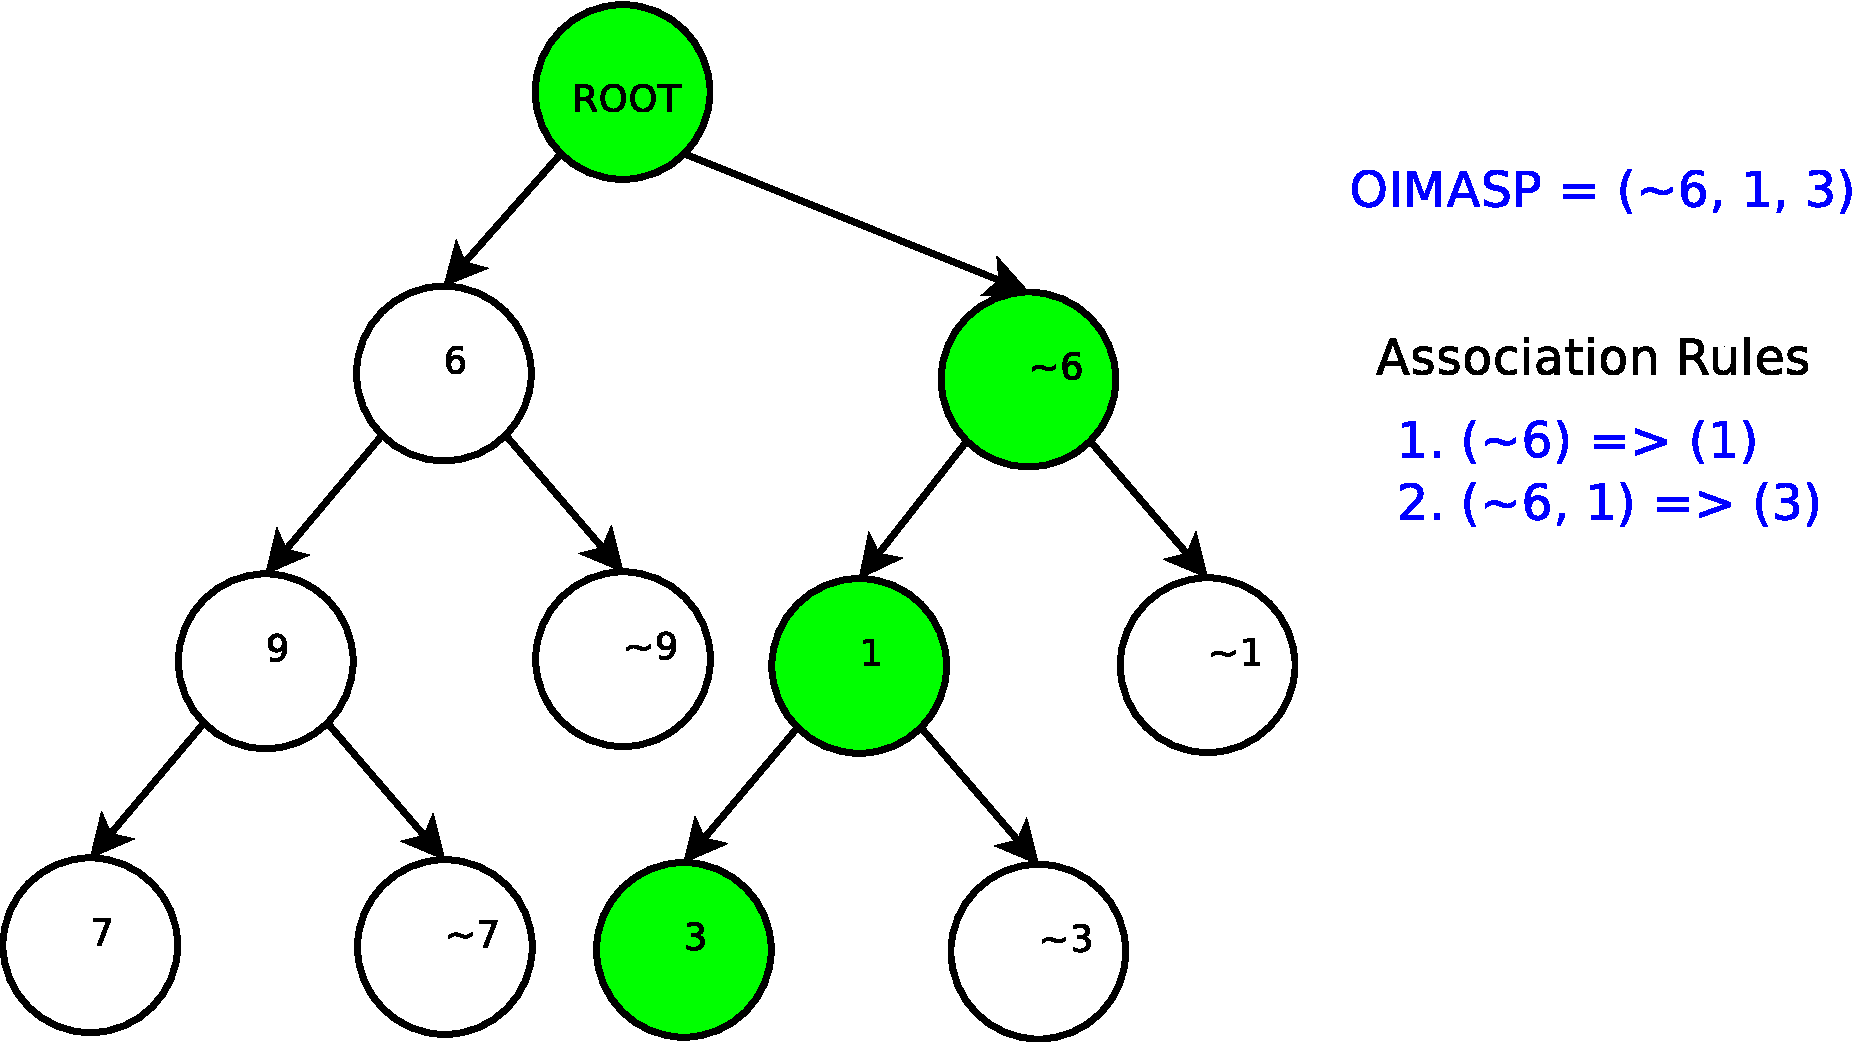
\includegraphics[scale=0.35]{pdf/oimasp}
\end{center}
\caption{An OIMASP(in green) and corresponding association rules}
\label{Fig 7}
\end{figure*}

\subsection{Modified version of OIMASP(OOIMASP) which takes into account origins of items in the transaction database}
In this section, we will discuss our second contribution which is addressed by modifying the \emph{MASP} algorithm proposed in \cite{oldmasp}. What if we want to generate those association rules which contains item $ I $? Our idea is to find the row starting from the top row of the transaction dataset in which item $ I $ appears for the first time(say $ ith $ row). Then for generating the $ OIMASP $ tree, we will consider $ ith $ transaction and transactions there after. Then we generate all the association rules and add only those rules to the solution set which contains item $ I $. It can be done for every unique element of $ \Gamma $ and finally take the union of solution sets obtained for each unique items to get the global solution set of association rules.

We will apply this algorithm for transaction dataset in Figure \ref{Fig 5}, threshold support($ \tau _{s} $) $ = 0.2 $, threshold confidence($ \tau _{c} $) $ = 0.3 $ and item $ = 10 $.

\begin{figure*}
\begin{center}
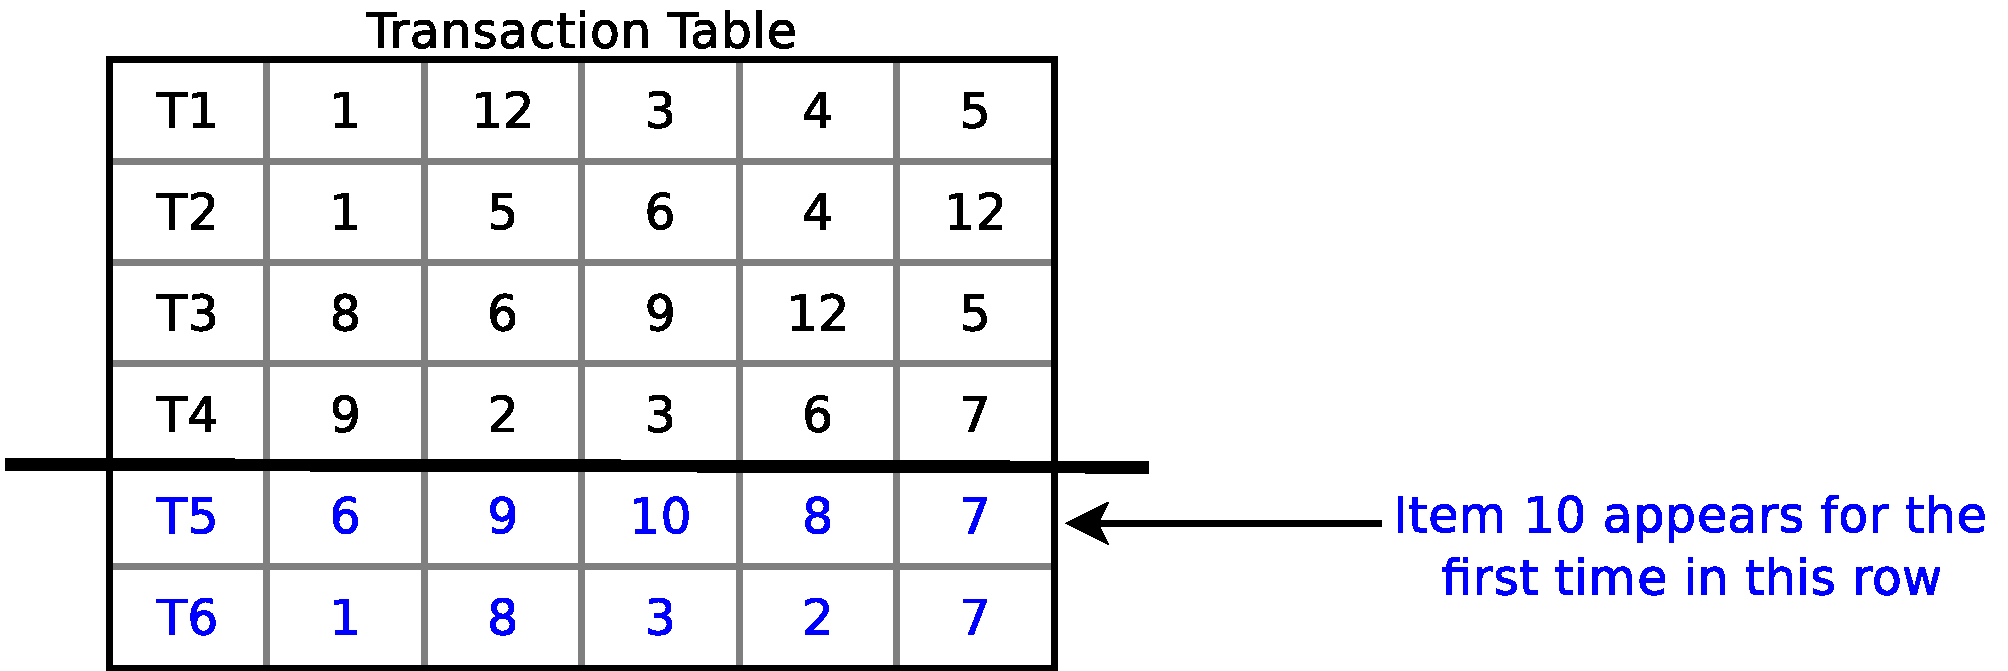
\includegraphics[scale=0.35]{pdf/partition}
\end{center}
\caption{Partition of dataset based on the origin of item $ 10 $}
\label{Fig 8}
\end{figure*}

\begin{figure}
\begin{center}
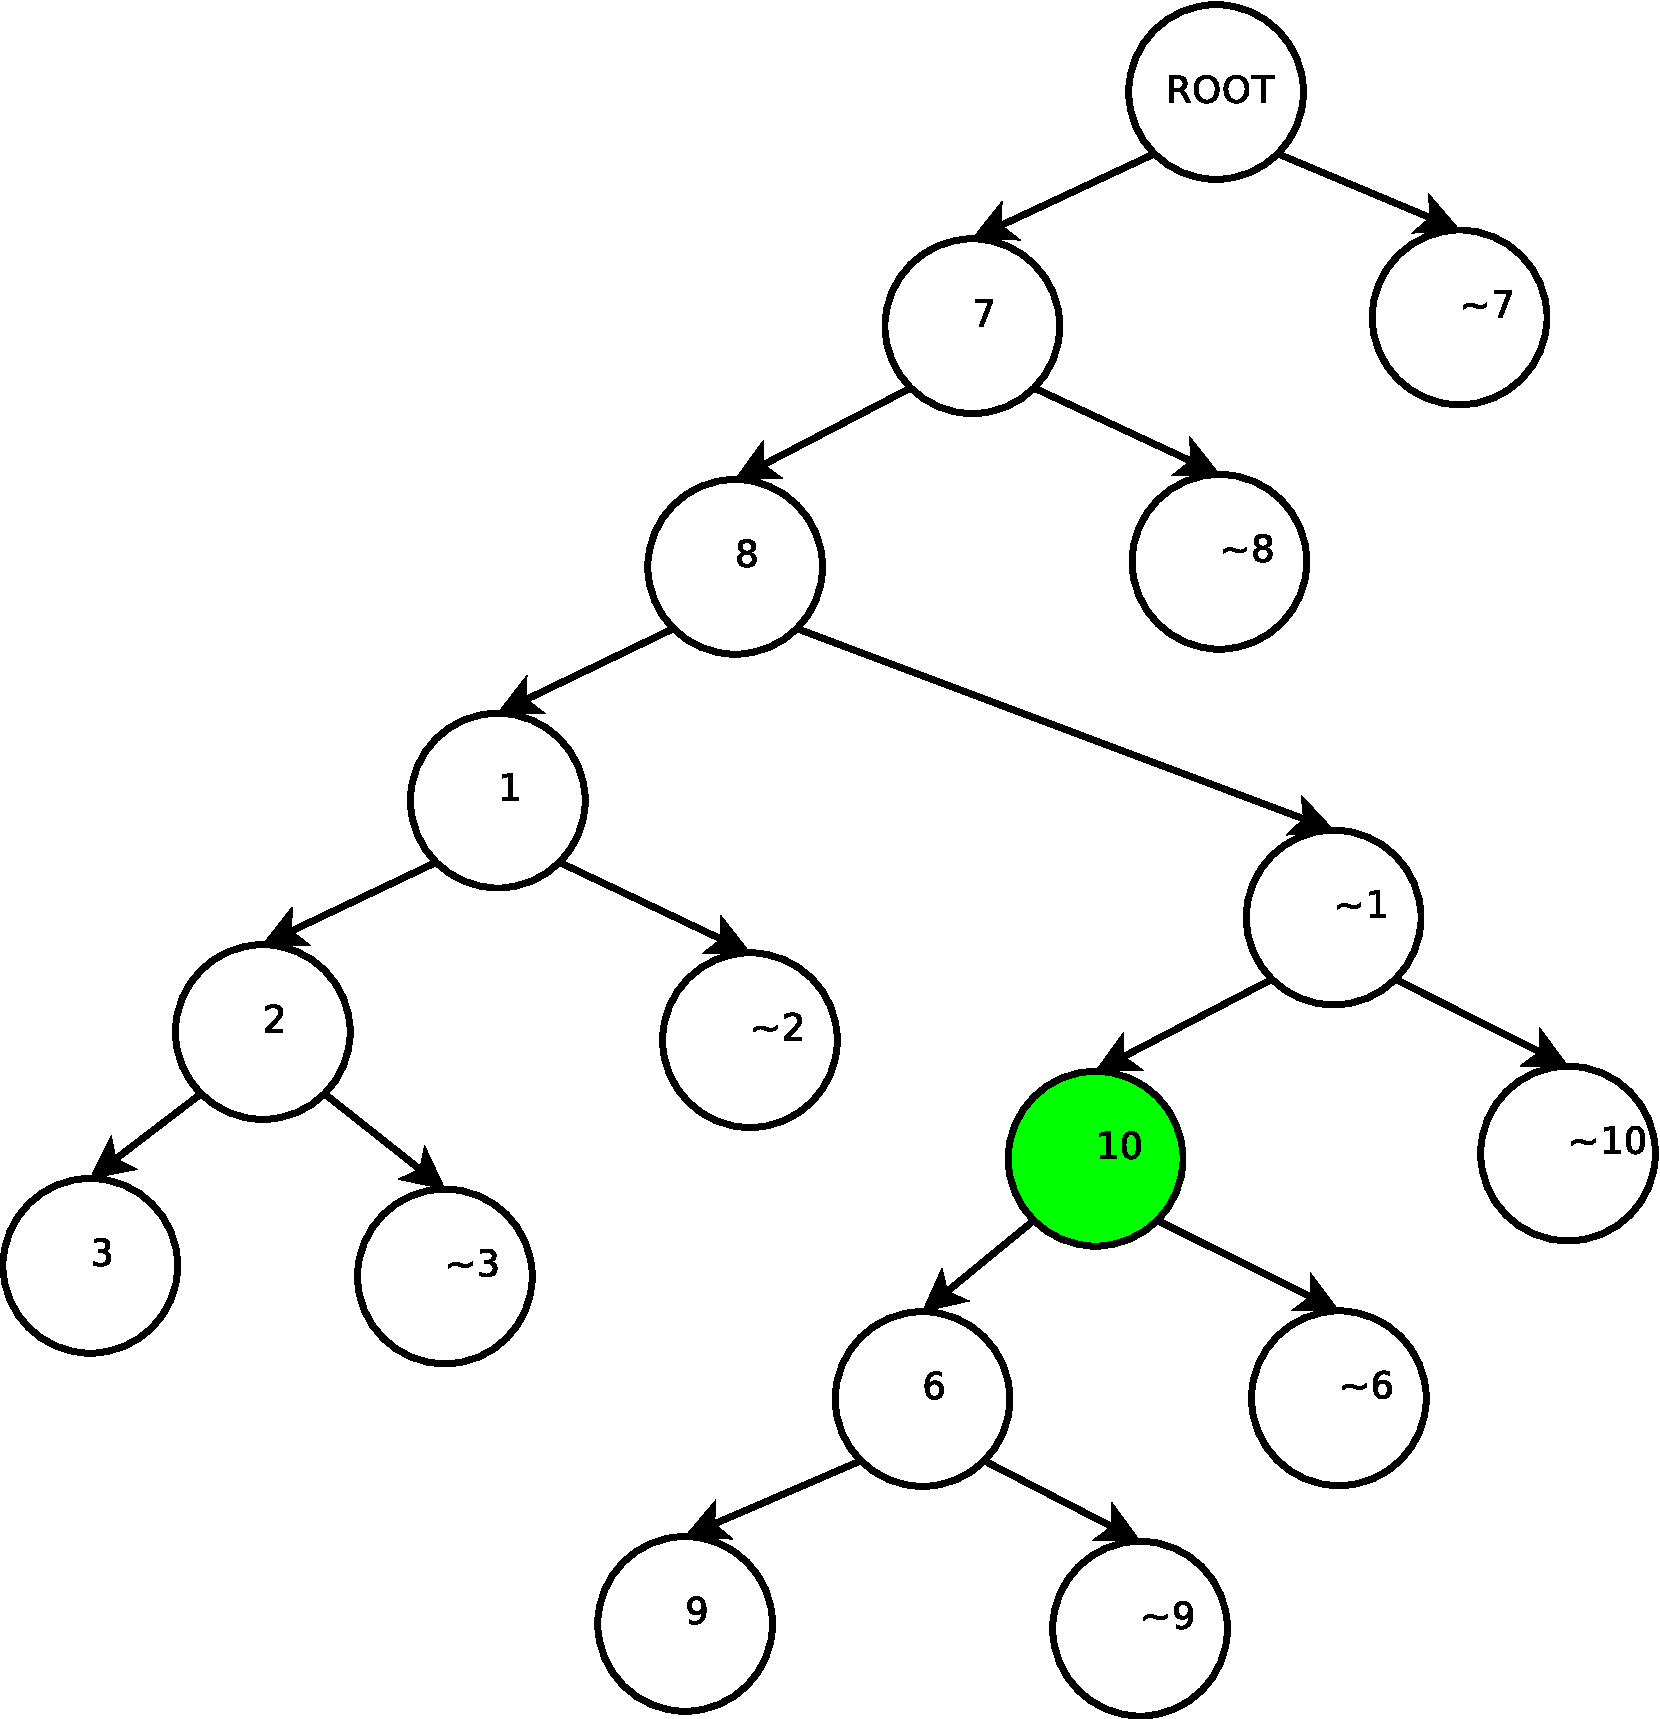
\includegraphics[scale=0.25]{pdf/moimasp}
\end{center}
\caption{An OIMASP tree}
\label{Fig 9}
\end{figure}

\begin{enumerate}[Step 1.]
\item A subdataset(consists of $ 5th $ and $ 6th $ row as shown in Figure \ref{Fig 8}) is obtained based on the origin of item $ 10 $.
\item Apply \emph{OIMASP} tree generation algorithm on the new dataset to obtain an OIMASP tree as shown in Figure \ref{Fig 9}.
\item Find association rules which conains item $ 10 $(Figure \ref{Fig 10}). Add rules obtained to the global solution set.
\item Repeat these steps for other items too.
\end{enumerate}

For the OIMASP tree in Figure \ref{Fig 9}, generate association rules for all $ OIMASPs $ having item $ 10 $(as done in Figure \ref{Fig 7}) and discard those rules which do not contain item $ 10 $ to obtain final ruleset as shown in Figure \ref{Fig 10}.

\begin{figure}
\begin{center}
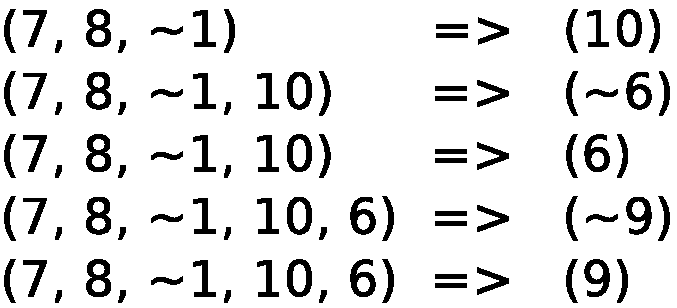
\includegraphics[scale=0.35]{pdf/arules10}
\end{center}
\caption{Association rules containing item $ 10 $}
\label{Fig 10}
\end{figure}

\textbf{Discussion:} If we generate $ OIMASP $ tree for all the items in the transaction database, then $ OIMASP $ tree generation algorithm will be called multiple numbers of times($ = $number of unique items in the dataset). It is possible that multiple items may have the same origin hence no need for redundancy(same $ OIMASP $ tree generation multiple times). Avoiding the redundancy can lead to fewer $ OIMASP $ tree productions. In the worst case, $ N $(total number of transactions) OIMASP trees will be generated.

\begin{algorithm}
    \SetKwInOut{Input}{Input}
    \SetKwInOut{Output}{Output}

    \underline{function OOIMASP} $ (\Gamma, \tau _{s}, \tau _{c}) $\;
    \Input{A transaction dataset $ \Gamma [N][M] $, threshold support $ \tau _{s} $ and 
	       threshold confidence $ \tau _{c} $}
    \Output{$ association\ rules $}
       
    $ items[1:j] $ $ \leftarrow $ unique items list \\
    $ origins[1:j] $ $ \leftarrow $ origin of corresponding items in $ items $ \\       
    $ globalRules \leftarrow \lbrace \rbrace $
       
	\For{i in 1 : j}
	  {
		$ currentItem $ $ \leftarrow $ $ items[i] $ \\
		$ itemOrigin $ $ \leftarrow $ $ origins[i] $ \\
			  	
	  	\If{$ OIMASP $ tree is not yet generated for origin $ itemOrigin $}
      	  {
            generate $ OIMASP $ tree for dataset $ = $ $ \Gamma[itemOrigin:N] $ and given $ \tau _{s} $, $ 				\tau _{c} $
          }	
          
		generate all association rules from $ OIMASP $ tree having origin $ = itemOrigin $, which contains 			item $ currentItem $ and add these to $ globalRules $
	  }
	          		
	return $ globalRules $;      
    \caption{OOIMASP Algorithm}
\end{algorithm}

\subsection{Complexity of OOIMASP algorithm}
The complexity of the \emph{MASP} algorithm \cite{oldmasp} is $ \Theta(NMlog(NM)) $. After the first improvement(OIMASP) complexity remains the same. In the concluding algorithm(\emph{OOIMASP}) \emph{OIMASP} can be called at max N times so that the complexity will be $ \displaystyle\sum_{i=1}^{N} \Theta(iMlog(iM)) = \Theta(N^{2}Mlog(NM)) $.

\section{Experimental setup and results}

The old approach and the new approach are compared using five datasets\footnote{\label{datasetlink} https://github.com/cryptomanic/OOIMASP-datasets} namely A[6x5], B[20x20], C[40x40], D[100x100] and E[1000x1000]. Metrics used for comparison are maximum rule size and the total number of rules generated. The OOIMASP algorithm will generate at least those rules that are produced by MASP. The OOIMASP algorithm generates five additional rules compared to MASP for dataset A(12) for $ threshold $ $ support $ 60\% and $ threshold $ $ confidence $ 30\%. The rule having maximum lengh(4) belongs to new rules. The rule having the maximum length(4) belongs to the new ruleset. The proposed approach generates not only additional rules but also responsible for introducing bigger rules. Similarly, for dataset B, C, and D the number of additional rules generated are 224, 99, and 63 respectively. In the case of transaction dataset E, the old approach is unable to generate any rule whereas the new method produces a large number of rules.

As you can see in Figure \ref{Fig 11} that the new approach outperforms the old approach w.r.t number of rules generated and longest rule size. The amount of information obtained from the dataset has compensated the increase in time complexity.

\begin{figure*}
\begin{center}
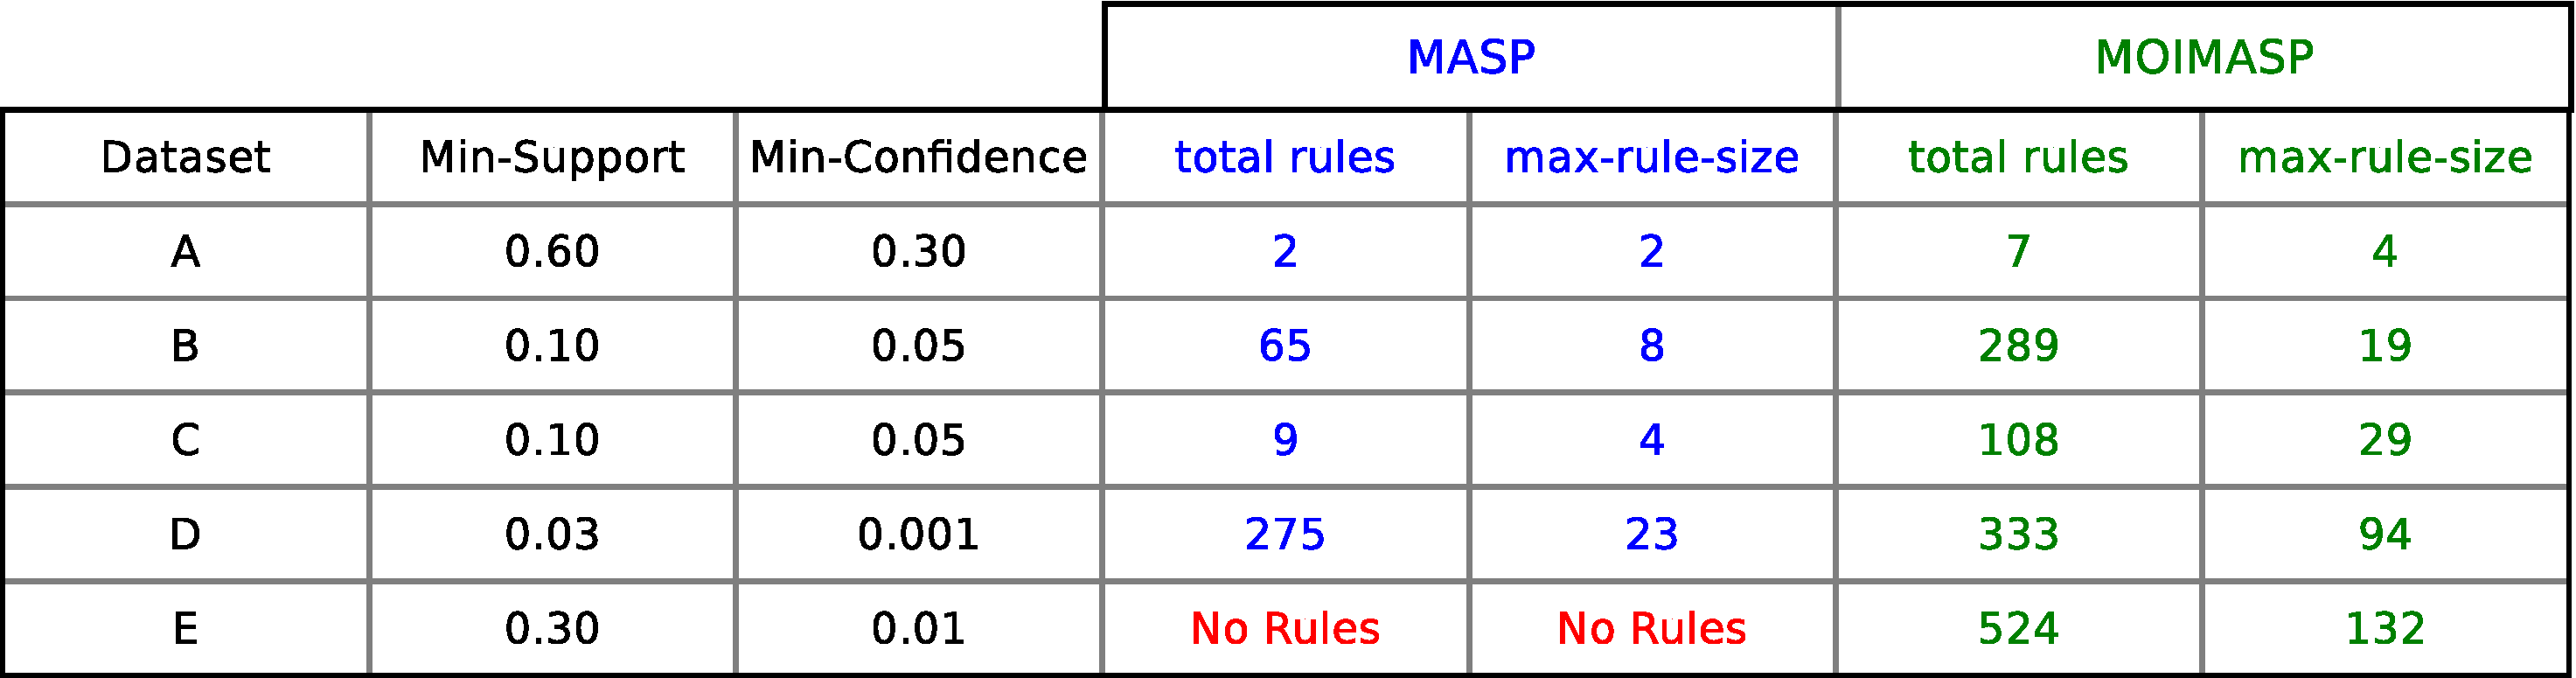
\includegraphics[scale=0.30]{pdf/comparison}
\end{center}
\caption{Comparison of \emph{MASP} and \emph{OOIMASP}}
\label{Fig 11}
\end{figure*}

\section{Conclusion}

\section*{References}

\bibliography{mybibfile}

\end{document}